\chapter{Experimentation Results and Discussion}


\hrule
\vspace{.5cm}
\section{Experimental Setup}
We have trained and tested above proposed model in google colaboratory, the feature engineering and machine learning algorithms were executed through the usage of the Pandas \cite{team2020pandas}, Scikit-learn libraries in Python. In addition to that, the hyperparameter optimization (HPO) techniques were implemented by utilization of the Skopt \cite{head2018scikit}, Hyperopt \cite{komer2014hyperopt} and Optuna libraries.

\par The experiments focus on the assessment of known cyber-attacks through labeled datasets, and focus on unknown cyber-attacks by using unlabeled datasets.

\pagebreak
\section{Datasets Description}
\subsection{CAN-intrusion-dataset}
The authors in \cite{seo2018gids} have introduced a method for detecting intrusions by analyzing the offset ratio and time interval between request and response messages in Controller Area Network (CAN). When a remote frame with a specific identifier is sent, a receiving node is expected to respond promptly. As a result, each node maintains a consistent response offset ratio and time interval under normal conditions, but these values change when an attack occurs.This concept is utilised in detecting intrusion in the network.

The attack types of this dataset are shown in Table 4.1.

\begin{table}[htbp]
\centering
\begin{tabular}{|l|r|}
\hline
\textbf{Attack Type} & \textbf{\# of Messages} \\ \hline
DoS Attack & 656,579 \\ \hline
Fuzzy Attack & 591,990 \\ \hline
Impersonation Attack & 995,472 \\ \hline
Attack-Free State & 2,369,868 \\ \hline
\end{tabular}
\caption{Distribution of Messages by Attack Type}
\label{tab:attack_messages}
\end{table}

\subsection{CICIDS2017 dataset}
The Canadian Institute for Cybersecurity Intrusion Detection Evaluation Dataset (CICIDS) is a publicly available dataset widely used for research and benchmarking in the field of intrusion detection systems (IDS). The dataset comprises a comprehensive collection of network traffic data, meticulously labeled with various types of cyber threats and anomalies as shown in Table 4.2 , Table 4.3 and Table 4.4 .The dataset contains most realistic and upto date data on different cyber attacks.The detailed analysis of this dataset is given in \cite{sharafaldin2019detailed}.

\begin{table}[htbp]
\centering
\caption{Features of CICIDS2017 dataset}
\begin{tabular}{|p{4cm}|p{6cm}|p{4cm}|}
\hline
\multicolumn{1}{|c|}{\textbf{Basic Flow Features}} & \multicolumn{1}{c|}{\textbf{Flow Statistics}} & \multicolumn{1}{c|}{\textbf{Packet Length Statistics}} \\
\hline
'Flow Duration' & 'Total Fwd Packets' & 'Fwd Packet Length Max' \\
 & 'Total Backward Packets' & 'Fwd Packet Length Min' \\
 & 'Total Length of Fwd Packets' & 'Fwd Packet Length Mean' \\
 & 'Total Length of Bwd Packets' & 'Fwd Packet Length Std' \\
 &  & 'Bwd Packet Length Max' \\
 &  & 'Bwd Packet Length Min' \\
 &  & 'Bwd Packet Length Mean' \\
 &  & 'Bwd Packet Length Std' \\
 & 'Flow Bytes/s' & 'Min Packet Length' \\
 & 'Flow Packets/s' & 'Max Packet Length' \\
 &  & 'Packet Length Mean' \\
 &  & 'Packet Length Std' \\
 &  & 'Packet Length Variance' \\
\hline
\multicolumn{1}{|c|}{\textbf{Inter-Arrival Times}} & \multicolumn{1}{c|}{\textbf{TCP Flags}} & \multicolumn{1}{c|}{\textbf{Packet Size Statistics}} \\
\hline
'Flow IAT Mean' & 'FIN Flag Count' & 'Average Packet Size' \\
'Flow IAT Std' & 'SYN Flag Count' & 'Avg Fwd Segment Size' \\
'Flow IAT Max' & 'RST Flag Count' & 'Avg Bwd Segment Size' \\
'Fwd IAT Total' & 'PSH Flag Count' &  \\
'Fwd IAT Mean' & 'ACK Flag Count' &  \\
'Fwd IAT Max' & 'ECE Flag Count' &  \\
'Fwd IAT Min' &  &  \\
'Bwd IAT Total' &  &  \\
'Bwd IAT Mean' &  &  \\
'Bwd IAT Std' &  &  \\
'Bwd IAT Max' &  &  \\
'Bwd IAT Min' &  &  \\
'Bwd PSH Flags' &  &  \\
'Fwd URG Flags' &  &  \\
\hline
\multicolumn{1}{|c|}{\textbf{Header Information}} & \multicolumn{1}{c|}{\textbf{Bulk Rate Statistics}} & \multicolumn{1}{c|}{\textbf{Other Features}} \\
\hline
'Bwd Header Length' & 'Fwd Avg Bytes/Bulk' & 'Init Win bytes forward' \\
'Fwd Packets/s' & 'Fwd Avg Packets/Bulk' & 'Init Win bytes backward' \\
'Bwd Packets/s' & 'Bwd Avg Bytes/Bulk' & 'act\_data\_pkt\_fwd' \\
 & 'Bwd Avg Bulk Rate' & 'min\_seg\_size\_forward' \\
 & 'Subflow Fwd Packets' & 'Active Mean' \\
 & 'Subflow Bwd Packets' & 'Active Std' \\
 & 'Subflow Bwd Bytes' & 'Active Max' \\
 &  & 'Active Min' \\
 &  & 'Idle Mean' \\
 &  & 'Idle Std' \\
 &  & 'Idle Max' \\
\hline
\end{tabular}
\end{table}

\begin{table}[htbp]
\centering
\begin{tabular}{|l|r|}
\hline
\textbf{Attack Type} & \textbf{Number of Data Points} \\ \hline
DoS Attack & 459,027 \\ 
DDoS Attack & 320,515 \\ 
Heartbleed Attack & 11,366 \\ 
Web Attack & 218,459 \\ 
Infiltration Attack & 36,102 \\ 
Botnet Attack & 1,048,586 \\ 
Port Scan & 158,930 \\ 
FTP Brute Force & 193,360 \\ 
SSH Brute Force & 200,755 \\ 
Brute Force & 155,100 \\ 
SQL Injection & 87,821 \\ 
Benign (Normal) & 2,540,047 \\ \hline
\textbf{Total} & \textbf{5,829,088} \\ \hline
\end{tabular}
\caption{Distribution of Attacks and Benign Traffic in CICIDS2017 Dataset}
\label{tab:attack_distribution}
\end{table}

\begin{table}[htbp]
\centering
\caption{Class distribution of CICIDS2017 dataset}
\begin{tabular}{lcl}
\toprule
\textbf{Category} & \textbf{Class labels} & \textbf{Attacks} \\
\midrule
Benign & 0 & Benign \\
\midrule
DoS/DDoS & 1 & Heartbleed, DDoS \\
         & & DoS Hulk, DoS GoldenEye \\
         & & DoS Slowloris, DoS Slowhttptest \\
\midrule
PortScan & 2 & PortScan \\
\midrule
Brute Force & 3 & FTP-Patator, SSH-Patator \\
\midrule
Web Attack & 4 & Web Attack -- Brute Force \\
           & & Web Attack -- XSS \\
           & &Web Attack -- SQL Injection \\
\midrule
Botnet & 5 & Bot \\
\midrule
Others & 6 & Unknown \\
\bottomrule
\end{tabular}
\end{table}

\pagebreak
\section{Performance analysis of Model}
To evaluate the performance of the ML models used in our proposed framework, we have used labeled datasets which represent intra vehicular network and extra vehicular network data.We have trained and tested the models on CICIDS2017 dataset and the validation metrics of those models are compared before and after hyper parameter tuning.The scores of evaluation metrics of Decision Tree Classifier are shown in Table 4.5.
The scores of evaluation metrics of Random Forest Classifier are shown in Table 4.6.
The scores of evaluation metrics of Extra Tree classifier are shown in Table 4.7. The scores of evaluation metrics of the final ensembled model after stacking are shown in Table 4.8.
We can conclude that accuracy scores of all the models have increased after performing Hyperparameter Optimization through Bayesian Optimization (BO).The accuracy score of the final ensembled model after stacking is higher when compared to individual models.These accuracy comparisons can be seen in Table 4.9.The miscalculation rate of the final ensembled model after hyperparameter optimization is 0.223880597 ,i.e,(1-accuracy).

\par Confusion matrix, a table used in classification to evaluate the performance of a ML model.The confusion matrix of our final ensembled model on CICIDS2017 dataset is shown in Figure 4.1.

% \begin{figure}[htbp]
% \centerline{\includegraphics[width=0.7 \textwidth]
% {img/features.jpg}}
% \caption{Features of CICIDS2017 dataset}
% \label{fig}
% \end{figure}

% \begin{table}[htbp]
% \centering
% \caption{Network Traffic Features}
% \begin{tabular}{p{4cm}|p{4cm}|p{4cm}}
% \hline
% \multicolumn{1}{c|}{\textbf{Basic Flow Features}} & \multicolumn{1}{c|}{\textbf{Flow Statistics}} & \multicolumn{1}{c}{\textbf{Packet Length Statistics}} \\
% \hline
% 'Flow Duration' & 'Total Fwd Packets' & 'Fwd Packet Length Max' \\
%  & 'Total Backward Packets' & 'Fwd Packet Length Min' \\
%  & 'Total Length of Fwd Packets' & 'Fwd Packet Length Mean' \\
%  & 'Total Length of Bwd Packets' & 'Fwd Packet Length Std' \\
%  &  & 'Bwd Packet Length Max' \\
%  &  & 'Bwd Packet Length Min' \\
%  &  & 'Bwd Packet Length Mean' \\
%  &  & 'Bwd Packet Length Std' \\
%  & 'Flow Bytes/s' & 'Min Packet Length' \\
%  & 'Flow Packets/s' & 'Max Packet Length' \\
%  &  & 'Packet Length Mean' \\
%  &  & 'Packet Length Std' \\
%  &  & 'Packet Length Variance' \\
% \hline
% \multicolumn{1}{c|}{\textbf{Inter-Arrival Times}} & \multicolumn{1}{c|}{\textbf{TCP Flags}} & \multicolumn{1}{c}{\textbf{Packet Size Statistics}} \\
% \hline
% 'Flow IAT Mean' & 'FIN Flag Count' & 'Average Packet Size' \\
% 'Flow IAT Std' & 'SYN Flag Count' & 'Avg Fwd Segment Size' \\
% 'Flow IAT Max' & 'RST Flag Count' & 'Avg Bwd Segment Size' \\
% 'Fwd IAT Total' & 'PSH Flag Count' &  \\
% 'Fwd IAT Mean' & 'ACK Flag Count' &  \\
% 'Fwd IAT Max' & 'ECE Flag Count' &  \\
% 'Fwd IAT Min' &  &  \\
% 'Bwd IAT Total' &  &  \\
% 'Bwd IAT Mean' &  &  \\
% 'Bwd IAT Std' &  &  \\
% 'Bwd IAT Max' &  &  \\
% 'Bwd IAT Min' &  &  \\
% 'Bwd PSH Flags' &  &  \\
% 'Fwd URG Flags' &  &  \\
% \hline
% \multicolumn{1}{c|}{\textbf{Header Information}} & \multicolumn{1}{c|}{\textbf{Bulk Rate Statistics}} & \multicolumn{1}{c}{\textbf{Other Features}} \\
% \hline
% 'Bwd Header Length' & 'Fwd Avg Bytes/Bulk' & 'Init Win bytes forward' \\
% 'Fwd Packets/s' & 'Fwd Avg Packets/Bulk' & 'Init Win bytes backward' \\
% 'Bwd Packets/s' & 'Bwd Avg Bytes/Bulk' & 'act\_data\_pkt\_fwd' \\
%  & 'Bwd Avg Bulk Rate' & 'min\_seg\_size\_forward' \\
%  & 'Subflow Fwd Packets' & 'Active Mean' \\
%  & 'Subflow Bwd Packets' & 'Active Std' \\
%  & 'Subflow Bwd Bytes' & 'Active Max' \\
%  &  & 'Active Min' \\
%  &  & 'Idle Mean' \\
%  &  & 'Idle Std' \\
%  &  & 'Idle Max' \\
% \hline
% \end{tabular}
% \end{table}

\begin{table}[htbp]
\centering
\caption{Metrics evaluation scores for Decision Tree Classifier}
\resizebox{0.8\textwidth}{!}{%
\begin{tabular}{|l|c|c|}
\hline
\textbf{Validation metric} & \textbf{Before Tuning} & \textbf{After Tuning}\\
\hline
Accuracy & 0.9929104477611941 & 0.9934701492537313\\
\hline
Precision & 0.9929326683116145 & 0.9934820633911605\\
\hline
Recall & 0.9929104477611941 & 0.9934701492537313\\
\hline
F1-score & 0.992915558827126 & 0.9934703509590384\\
\hline
\end{tabular}%
}
\end{table}

\begin{table}[htbp]
\centering
\caption{Metrics evaluation scores for Random Forest Classifier}
\resizebox{0.8\textwidth}{!}{%
\begin{tabular}{|l|c|c|}
\hline
\textbf{Validation metric} & \textbf{Before Tuning} & \textbf{After Tuning}\\
\hline
Accuracy & 0.9958955223880597 & 0.9970149253731343\\
\hline
Precision & 0.995905600456217 & 0.9970229763459072\\
\hline
Recall & 0.9958955223880597 & 0.9970149253731343\\
\hline
F1-score & 0.9958667158915585 & 0.9969855634666102\\
\hline
\end{tabular}%
}
\end{table}

\begin{table}[htbp]
\centering
\caption{Metrics evaluation scores for Evaluation Tree Classifier}
\resizebox{0.8\textwidth}{!}{%
\begin{tabular}{|l|c|c|}
\hline
\textbf{Validation metric} & \textbf{Before Tuning} & \textbf{After Tuning}\\
\hline
Accuracy & 0.9934701492537313 & 0.996268656716418\\
\hline
Precision & 0.9934936993097583 & 0.9962809018799189\\
\hline
Recall & 0.9934701492537313 & 0.996268656716418\\
\hline
F1-score & 0.9934001720288478 & 0.9962399897437341\\
\hline
\end{tabular}%
}
\end{table}

\begin{table}[htbp]
\centering
\caption{Metrics evaluation scores for Ensembled Model after Stacking}
\resizebox{0.8\textwidth}{!}{%
\begin{tabular}{|l|c|c|}
\hline
\textbf{Validation metric} & \textbf{Before Tuning} & \textbf{After Tuning}\\
\hline
Accuracy & 0.9958955223880597 & 0.9977611940298508\\
\hline
Precision & 0.9959068447137124 & 0.9977637524166587\\
\hline
Recall & 0.9958955223880597 & 0.9977611940298508\\
\hline
F1-score & 0.9958973352521118 & 0.9976686498123707\\
\hline
\end{tabular}%
}
\end{table}



\begin{table}[htbp]
\centering
\caption{Accuracy comparisons on various models}
\resizebox{0.8\textwidth}{!}{%
\begin{tabular}{|l|c|c|}
\hline
\textbf{Accuracy} & \textbf{Before Tuning} & \textbf{After Tuning}\\
\hline
\textbf{ML Model} & & \\
\hline
Decision Tree & 0.9929104477611941 & 0.9934701492537313\\
\hline
Random Forest & 0.9958955223880597 & 0.9970149253731343\\
\hline
Extra Tree & 0.9934701492537313 & 0.996268656716418\\
\hline
Final Ensembled Model after Stacking & 0.9958955223880597 & 0.9977611940298508\\
\hline
\end{tabular}%
}
\end{table}

\pagebreak
\begin{table}[htbp]
\centering
\caption{Performance of Overall model}
\resizebox{0.8\textwidth}{!}{%
\begin{tabular}{|c|c|c|c|c|}
\hline
\textbf{Class label} & \textbf{Precision} & \textbf{Recall} & \textbf{F1-score} & \textbf{Support} \\
\hline
0 & 1.00 & 1.00 & 1.00 & 3655 \\
1 & 0.99 & 0.99 & 0.99 & 385 \\
2 & 1.00 & 1.00 & 1.00 & 19 \\
3 & 1.00 & 1.00 & 1.00 & 605 \\
4 & 1.00 & 0.50 & 0.67 & 6 \\
5 & 1.00 & 1.00 & 1.00 & 256 \\
6 & 1.00 & 1.00 & 1.00 & 434 \\
\hline
% Accuracy & & & 1.00 & 5360 \\
% Macro Average & 1.00 & 0.93 & 0.95 & 5360 \\
% Weighted Average & 1.00 & 1.00 & 1.00 & 5369 \\
% \hline
\end{tabular}%
}
\end{table}




\begin{figure}[htbp]
\centerline{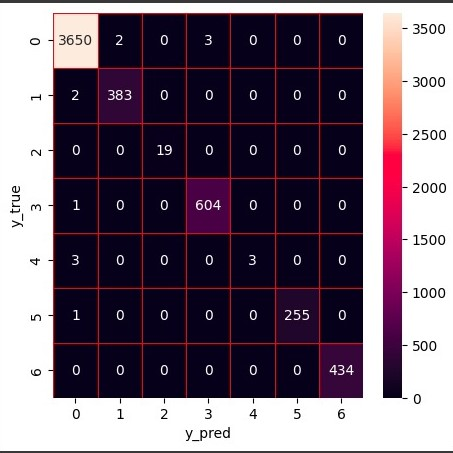
\includegraphics[width=0.7\textwidth]{img/confusion_matrix.jpg}}
\caption{Confusion matrix}
\label{fig}
\end{figure}

% \begin{table}[htbp]
%     \centering
%     \caption{Metrics evaluation scores for Decision Tree Classifier}
%     \resizebox{0.8\textwidth}{!}{%
%     \begin{tabular}{|l|c|c|}
%     \hline
%     \textbf{Validation metric} & \textbf{Before Tuning} & \textbf{After Tuning}\\ 
%     \hline
%     Accuracy & 0.9929104477611941 & 0.9934701492537313\\
%     \hline
%     Precision & 0.9929326683116145 & 0.9934820633911605\\
%     \hline
%     Recall & 0.9929104477611941 & 0.9934701492537313\\
%     \hline
%     F1-score & 0.992915558827126 & 0.9934703509590384\\
%     \hline
%     \end{tabular}%
%     }
% \end{table}


% \begin{table}[htbp]
%     \centering
%     \caption{Metrics evaluation scores for Random Forest Classifier}
%     \resizebox{0.8\textwidth}{!}{%
%     \begin{tabular}{|l|c|c|}
%     \hline
%     \textbf{Validation metric} & \textbf{Before Tuning} & \textbf{After Tuning}\\ 
%     \hline
%     Accuracy & 0.9958955223880597 & 0.9970149253731343\\
%     \hline
%     Precision & 0.995905600456217 & 0.9970229763459072\\
%     \hline
%     Recall & 0.9958955223880597 & 0.9970149253731343\\
%     \hline
%     F1-score & 0.9958667158915585 & 0.9969855634666102\\
%     \hline
%     \end{tabular}%
%     }
% \end{table}


% \begin{table}[htbp]
%     \centering
%     \caption{Metrics evaluation scores for Evaluation Tree Classifier}
%     \resizebox{0.8\textwidth}{!}{%
%     \begin{tabular}{|l|c|c|}
%     \hline
%     \textbf{Validation metric} & \textbf{Before Tuning} & \textbf{After Tuning}\\ 
%     \hline
%     Accuracy & 0.9934701492537313 & 0.996268656716418\\
%     \hline
%     Precision & 0.9934936993097583 & 0.9962809018799189\\
%     \hline
%     Recall & 0.9934701492537313 & 0.996268656716418\\
%     \hline
%     F1-score & 0.9934001720288478 & 0.9962399897437341\\
%     \hline
%     \end{tabular}%
%     }
% \end{table}


% \begin{table}[htbp]
%     \centering
%     \caption{Metrics evaluation scores for Ensembled Model after Stacking}
%     \resizebox{0.8\textwidth}{!}{%
%     \begin{tabular}{|l|c|c|}
%     \hline
%     \textbf{Validation metric} & \textbf{Before Tuning} & \textbf{After Tuning}\\ 
%     \hline
%     Accuracy & 0.9958955223880597 & 0.9977611940298508\\
%     \hline
%     Precision & 0.9959068447137124 & 0.9977637524166587\\
%     \hline
%     Recall & 0.9958955223880597 & 0.9977611940298508\\
%     \hline
%     F1-score & 0.9958973352521118 & 0.9976686498123707\\
%     \hline
%     \end{tabular}%
%     }
% \end{table}

% \begin{table}[htbp]
%     \centering
%     \caption{Accuracy comparisons on various models}
%     \resizebox{0.8\textwidth}{!}{%
%     \begin{tabular}{|l|c|c|}
%     \hline
%     \textbf{Accuracy} & \textbf{Before Tuning} & \textbf{After Tuning}\\ 
%     \hline
%     \textbf{ML Model} & & \\ 
%     \hline
%     Decision Tree & 0.9929104477611941 & 0.9934701492537313\\
%     \hline
%     Random Forest & 0.9958955223880597 & 0.9970149253731343\\
%     \hline
%     Extra Tree & 0.9934701492537313 & 0.996268656716418\\
%     \hline
%     Final Ensembled Model after Stacking & 0.9958955223880597 & 0.9977611940298508\\
%     \hline
%     \end{tabular}%
%     }
% \end{table}


% \begin{figure}[htbp]
% \centerline{\includegraphics[width=0.7 \textwidth]
% {img/confusion_matrix.jpg}}
% \caption{Confusion matrix}
% \label{fig}
% \end{figure}


